% Gemini theme
% https://github.com/anishathalye/gemini

\documentclass[final]{beamer}

% ====================
% Packages
% ====================

\usepackage[polish]{babel}
\usepackage[T1]{fontenc}
\usepackage{lmodern}
\usepackage[orientation=portrait,size=a3,scale=1.15]{beamerposter}
\usetheme{gemini}
\usecolortheme{gemini}
\usepackage{graphicx}
\graphicspath{{./images/}}
\usepackage{booktabs}
\usepackage{tikz}
\usepackage{pgfplots}
\pgfplotsset{compat=1.14}
\usepackage{anyfontsize}
\usepackage[backend=biber,
        style=ieee,     % styl numeryczny IEEE prawie jak PN
        sorting=nyt,    % sortowanie spisu po nazwiskach
        citestyle=numeric-comp % kompaktowe odnośniki numeryczne typu [21-23]
    ]{biblatex}
\addbibresource{poster.bib}

% ====================
% Lengths
% ====================

% If you have N columns, choose \sepwidth and \colwidth such that
% (N+1)*\sepwidth + N*\colwidth = \paperwidth
\newlength{\sepwidth}
\newlength{\colwidth}
\setlength{\sepwidth}{0.025\paperwidth}
\setlength{\colwidth}{0.45\paperwidth}

\newcommand{\separatorcolumn}{\begin{column}{\sepwidth}\end{column}}

% ====================
% Title
% ====================

\title{Porównanie algorytmów kryptografii asymetrycznej i zastosowania}

\author{Krzysztof Dąbrowski, Hussein Hazime, \\ Krzysztof Rudnik, Piotr Szczerba,\\ Jakub Więcław}

% \institute[shortinst]{Wydział Elektryczny Politechniki Warszawskiej}

% ====================
% Footer (optional)
% ====================

\footercontent{
  \hfill
  \hfill
  
\includegraphics[height=1.5cm]{repo-qr-code}}
% (can be left out to remove footer)


% ====================
% Logo (optional)
% ====================

% use this to include logos on the left and/or right side of the header:
\logoright{
\includegraphics[height=2.5cm]{logos/WE-znak-1}}

% ====================
% Body
% ====================

\begin{document}

% Refer to https://github.com/k4rtik/uchicago-poster
% logo: https://www.cam.ac.uk/brand-resources/about-the-logo/logo-downloads
% \addtobeamertemplate{headline}{}
% {
%     \begin{tikzpicture}[remember picture,overlay]
%       \node [anchor=north west, inner sep=3cm] at ([xshift=-2.5cm,yshift=1.75cm]current page.north west)
%       {\includegraphics[height=7cm]{logos/unott-logo.eps}}; 
%     \end{tikzpicture}
% }

\begin{frame}[t]
\begin{columns}[t]
\separatorcolumn

\begin{column}{\colwidth}

  \begin{block}{Wprowadzenie}

Kryptografia asymetryczna to technika szyfrowania, która umożliwia bezpieczną komunikację przez niezaufane kanały.
Poufność komunikacji jest zapewniona dzięki wykorzystaniu par kluczy – publicznych, dostępnych dla wszystkich, oraz prywatnych, stanowiących osobiste sekrety właścicieli. Zazwyczaj jeden klucz służy do szyfrowania wiadomości, a drugi do jej odszyfrowania.
%Kryptografia asymetryczna towarzyszy nam niemal na każdym kroku wirtualnych podróży i stanowi jeden z filarów współczesnego cyberbezpieczeństwa.

  \end{block}

  \begin{block}{Matematyczne fundamenty kryptografii: Porównanie Algorytmów}




%PUZZLE MERKLE'A
\textbf{Puzzle Merkle'a:}\\[10px]
Puzzle Merkle’a to pierwsza publicznie przedstawiona metoda umożliwiająca bezpieczną komunikację przez niezaufane kanały \cite{MerklePuzzles}.
Schemat działania dla komunikacji Ali z Bobem wygląda następująco:
\begin{itemize}
\item Ala tworzy listę \( m \) zaszyfrowanych słabym kluczem \( k \) zagadek, każda zawiera identyfikator i mocny klucz \( K \).
\item Bob losowo wybiera jedną i łamie ją metodą brute force (\( n \) obliczeń), po czym przesyła Ali identyfikator.
\item Ala i bob mogą się komunikować szyfrując wiadomości kluczem \( K \)\\[10px]
\end{itemize}
W tym przypadku za klucz publiczny można uważać listę przesłaną przez Alę, a za klucz prywatny zagadkę wybraną przez Boba. Do złamania szyfru potrzeba średnio \( \frac{n \times m}{2} \) obliczeń. Ze względu na to, że stosunek pracy wymaganej od nadawcy i odbiorcy do pracy potrzebnej do złamania szyfru był zbyt wysoki, 
metoda ta nie znalazła szerokiego zastosowania w praktyce.

%RSA
% RSA i ECC to popularne algorytmy kryptograficzne oparte na kluczach publicznych, różniące się pod względem matematycznych podstaw i wydajności.

\textbf{Generowanie kluczy RSA:}

    \begin{wrapfigure}{}{\textwidth}
    \centering
    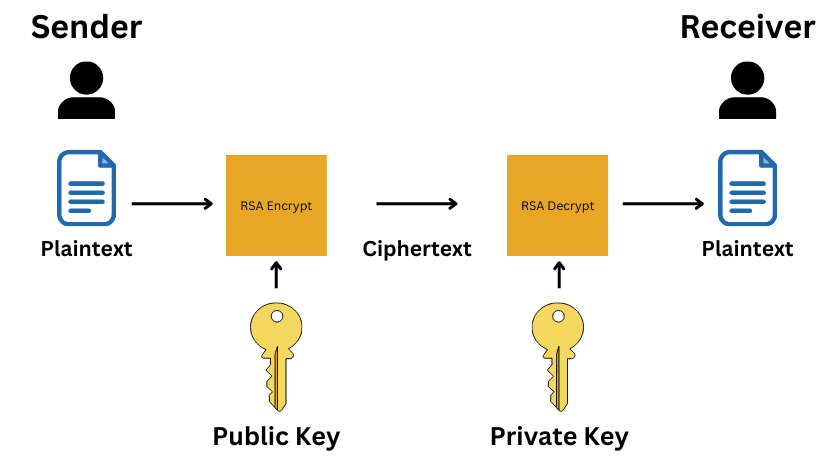
\includegraphics[width=0.975\textwidth]{images/rsa.png}
    % \caption{Schemat szyfrowania E2E}
    \label{fig:RSA}
    \end{wrapfigure}

\begin{itemize}
    \item Użytkownik, który chce wysłać/odebrać wiadomość, używa klucza publicznego/prywatnego \( (e, n) \) do zaszyfrowania/odszyfrowania wiadomości \( M \) :
    \[
    C = M^e \mod n  ; M = C^d \mod n
    \]
\end{itemize}

%\end{block}
%\begin{block}
 \textbf{Generowanie kluczy wykorzystując metodę ECC:}

Kryptografia krzywych eliptycznych (ECC) jest definiowana za pomocą następującego ogólnego równania:

\[
    y^2 = x^3 + ax + b
\]

gdzie $a$ i $b$ są współczynnikami krzywej eliptycznej.


Warunek $\Delta \neq 0$ zapewnia, że krzywa tworzy \textbf{grupę algebraiczną}, co jest konieczne do zastosowania jej w kryptografii. Jeśli $\Delta = 0$, struktura matematyczna krzywej nie jest prawidłowa do użycia w szyfrowaniu.
   
    \textbf{Generowanie klucza Użytkownika A:}
    \begin{itemize}
        \item Użytkownik A wybiera klucz prywatny $V_A$, gdzie $V_A < n$.
        \item Oblicza klucz publiczny $P_A(x, y) = V_A \times G(x, y)$.
    \end{itemize}

    \textbf{Generowanie klucza Użytkownik B:}
    \begin{itemize}
        \item Użytkownik B wybiera klucz prywatny $V_B$, gdzie $V_B < n$.
        \item Oblicza klucz publiczny $P_B(x, y) = V_B \times G(x, y)$.
    \end{itemize}

 

  \end{block}
\end{column}

\separatorcolumn

\begin{column}{\colwidth}  

\begin{block}{Kryptowaluty}
% \begin{center}
    
%         
\includegraphics[width=0.1\textwidth, height=0.1\textwidth ]{logos/images/graphics/Bitcoin.jpg} & 
\includegraphics[width=0.1\textwidth, height=0.1\textwidth]{logos/images/graphics/Ethereum.png} &
%         
\includegraphics[width=0.1\textwidth, height=0.1\textwidth]{logos/images/graphics/Dogecoin.png}  & \hspace{0.2cm} & 
\includegraphics[width=0.1\textwidth, height=0.1\textwidth]{logos/images/graphics/Litecoin.jpg} \\
% \end{center}
Kryptowaluty to cyfrowe waluty wykorzystujące kryptografię do zabezpieczania transakcji. Dzięki technologii blockchain możliwe jest prowadzenie transparentnej i bezpiecznej księgi transakcji bez potrzeby centralnego organu kontrolnego. Przykłady kryptowalut to Bitcoin, Ethereum i Dogecoin.
\end{block}

  \begin{alertblock}{Komunikatory E2E}
    \begin{wrapfigure}{}{\textwidth}
    \centering
    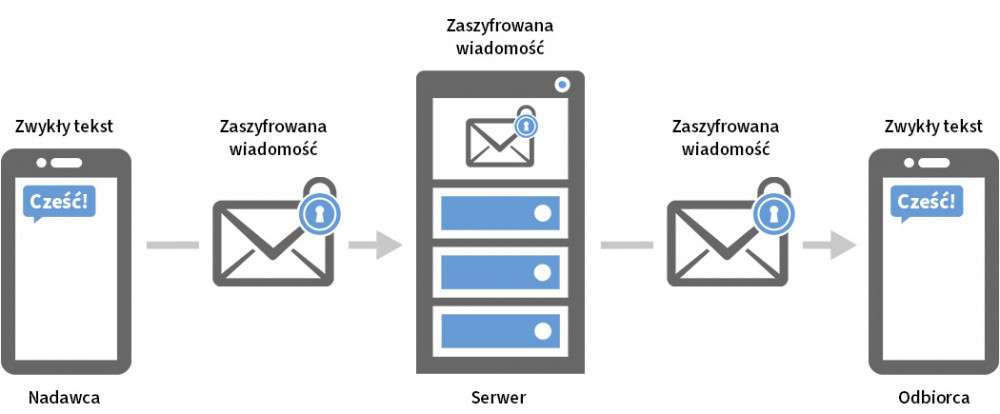
\includegraphics[width=0.975\textwidth]{logos/images/szyfrowanie-end-to-end.jpg}
    % \caption{Schemat szyfrowania E2E}
    \label{fig:e2e}
    \end{wrapfigure}
Komunikatory z szyfrowaniem end-to-end (E2E) zapewniają prywatność rozmów, ponieważ wiadomości są szyfrowane na urządzeniu nadawcy i odszyfrowywane dopiero na urządzeniu odbiorcy. Oznacza to, że nawet dostawca usługi nie ma dostępu do treści wiadomości. Popularne komunikatory E2E to m.in. Signal, WhatsApp czy Threema.
\end{alertblock}

    \begin{block}{Bezpieczeństwo tej samej długości klucza}

    Porównując bezpieczeństwo algorytmów kryptograficznych o tej samej długości klucza, kluczowy jest koncept bitów bezpieczeństwa \cite{BitSecurityOfCryptographicPrimitives}. Wartość ta określana jest jako: 
    $x = \log_2(N)$
    , gdzie \( N \) to średnia ilość operacji potrzebnych do złamania szyfru. Przykładowo, algorytm o sile 20 bitów bezpieczeństwa wymaga \( 2^{20} = 1048576 \) operacji do złamania \cite{BitSecurityOfCryptographicPrimitives}. 
    
    Dla RSA najszybszy klasyczny algorytm używany do ataków to Ogólne sito ciała liczbowego.
    W przypadku łamania ECC używany jest algorytm faktoryzacji rho Pollarda \cite{SolvingECDLP}.
    Wyliczając złożoność obliczeniową tych algorytmów, można przedstawić liczbę bitów bezpieczeństwa dla danej długości klucza.
    
    \begin{center}
        \includegraphics[width=\textwidth]{images/Porównanie bitów bezpieczeństwa dla danych kluczy RSA i ECC.png}
        \caption{Porównanie bitów bezpieczeństwa dla danych kluczy RSA i ECC}
    \end{center}

    \textbf{Wyraźnie mniejsza ilość bitów bezpieczeństwa algorytmu RSA dla danej długości klucza nie oznacza, że jest to niebezpieczny algorytm.} Trzeba jednak mieć na uwadze, że istotne jest użycie odpowiednio długiego klucza, by zapewnić bezpieczeństwo.

    \end{block}
 
  \begin{block}{Bibliografia}
    % \nocite{*}
    \footnotesize{\printbibliography}
  \end{block}

\end{column}
\separatorcolumn



\end{columns}
\end{frame}

\end{document}
